\begin{frame}
 \frametitle{Change of Coordinates}

  Change in original position and orientation $\to$ new coordinates

\pause

Example:
  \begin{itemize}
   \item Move ahead 1m;
   \item Turn a quarter of a circle to the right.
  \end{itemize}
  
%
\begin{table}[h]
\begin{tabular}{lcr}
  \psfrag{P}{$P(3,1,2)$}
  \psfrag{O}{$O(0,0,0)$}  
  \psfrag{x}{$x=3$} 
  \psfrag{y}{$y=1$} 
  \psfrag{z}{$z=2$}     
  \psfrag{A}{$Ox$}
  \psfrag{L}{$Oy$}
  \psfrag{U}{$Oz$}  
  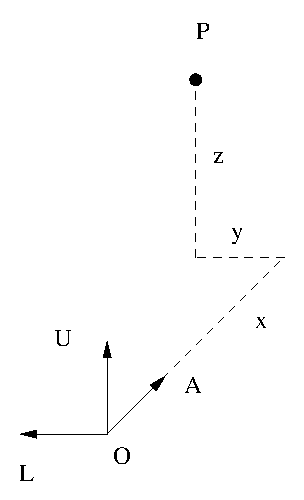
\includegraphics[height=2in]{./images/projector.eps}
%
& \hspace{2cm} &
%
\psfrag{P}{$P$}
  \psfrag{Op}{$O'$} 
  \psfrag{O}{$O$}  
  \psfrag{L}{$L$}
  \psfrag{U}{$U$}   
  \psfrag{xp}{$x'=-1$} 
  \psfrag{yp}{$y'=2$} 
  \psfrag{zp}{$z'=2$}     
  \psfrag{Ap}{$A'$}
  \psfrag{Lp}{$L'$}
  \psfrag{Up}{$U'$}  
  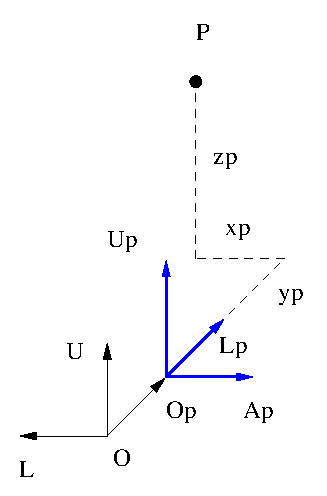
\includegraphics[height=2in]{./images/new_frame.eps}
%
\end{tabular}
  \end{table}
%  
%
\pause  
New coordinates of projector: $P \to (x',y',z') = (-1,2,2)$
\end{frame}

\begin{frame}
\frametitle{General formula for this change of coordinates}
%
\begin{table}[h]
\begin{tabular}{lcr}
  \psfrag{P}{$P(x,y,z)$}
  \psfrag{O}{$O(0,0,0)$}  
  \psfrag{x}{$x$} 
  \psfrag{y}{$y$} 
  \psfrag{z}{$z$}     
  \psfrag{A}{$Ox$}
  \psfrag{L}{$Oy$}
  \psfrag{U}{$Oz$}  
  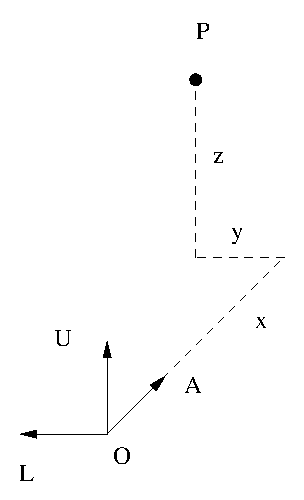
\includegraphics[height=2in]{./images/projector.eps}
%
& \hspace{2cm} &
%
\psfrag{P}{$P(x', y', z')$}
  \psfrag{Op}{$O'$} 
  \psfrag{O}{$O$}  
  \psfrag{L}{$L$}
  \psfrag{U}{$U$}   
  \psfrag{xp}{$x'=-y$} 
  \psfrag{yp}{$y'=x-1$} 
  \psfrag{zp}{$z'=z$}     
  \psfrag{Ap}{$A'$}
  \psfrag{Lp}{$L'$}
  \psfrag{Up}{$U'$}  
  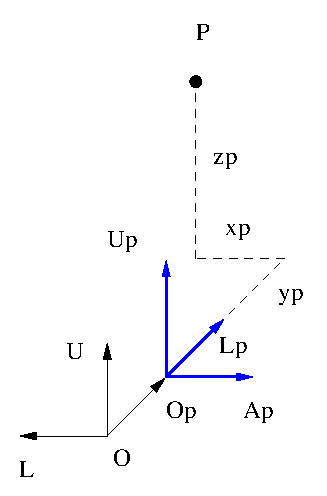
\includegraphics[height=2in]{./images/new_frame.eps}
%
\end{tabular}
  \end{table}
%  

\begin{eqnarray*}
 x' = & -y \\
 y' = & x-1 \\
 z' = & z
\end{eqnarray*}
%
Example $Q(x=1,y=2,z=3) \leftrightarrow Q(x'=-2, y'=0,z'=3)$

\end{frame}



\begin{frame}
 \frametitle{Fundamental Philosophy}
  $P(3,1,2)$ and $Q(1,2,3)$ in $(x,y,z)-$coordinates

  $P(-1,2,2)$ and $Q(-2,0,3)$ in $(x',y'z')-$coordinates

  Distance in new coordinates:
 \pause
%
$$d_{x',y',z'}(P,Q) = \sqrt{(-2+1)^2+(0-2)^2+(3-2)^2} = \sqrt{6} = d_{x,y,z}(P,Q)$$

Fundamental Philosophy:\pause
\begin{itemize}
 \item Space doesn't come with coordinates
  \item Natural concepts (such of distance) are independent of coordinates
  \item If a natural concept is defined using coordinates, \\
          the result does not depend on the chosen coordinate system.
\end{itemize}


\end{frame}